\documentclass[../notebook.tex]{subfiles}

\begin{document}
\nbentry{July 21, 2020}{%
  Computer generation of natural image elements
}

\subfile{../python-notebooks/tex/functional-graphics}

\begin{figure}[ht]
  \centering
  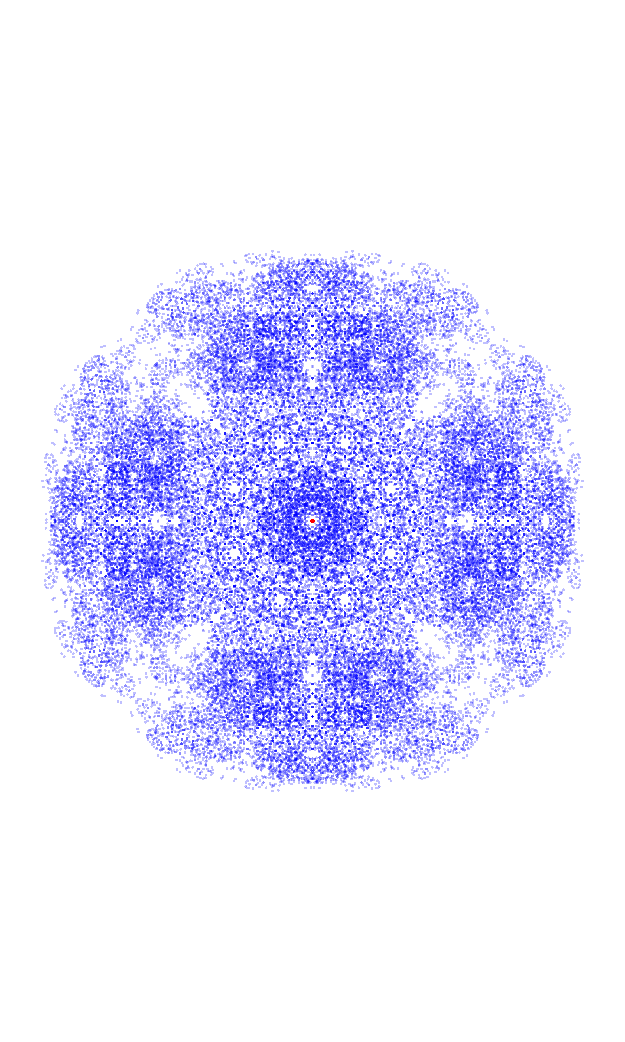
\includegraphics{../python-notebooks/mandala.pdf}
  \caption{Ma\d{n}\d{d}ala-like pattern from an iterated function system.}\label{fig:mandala}
\end{figure}
\begin{figure}[ht]
  \centering
  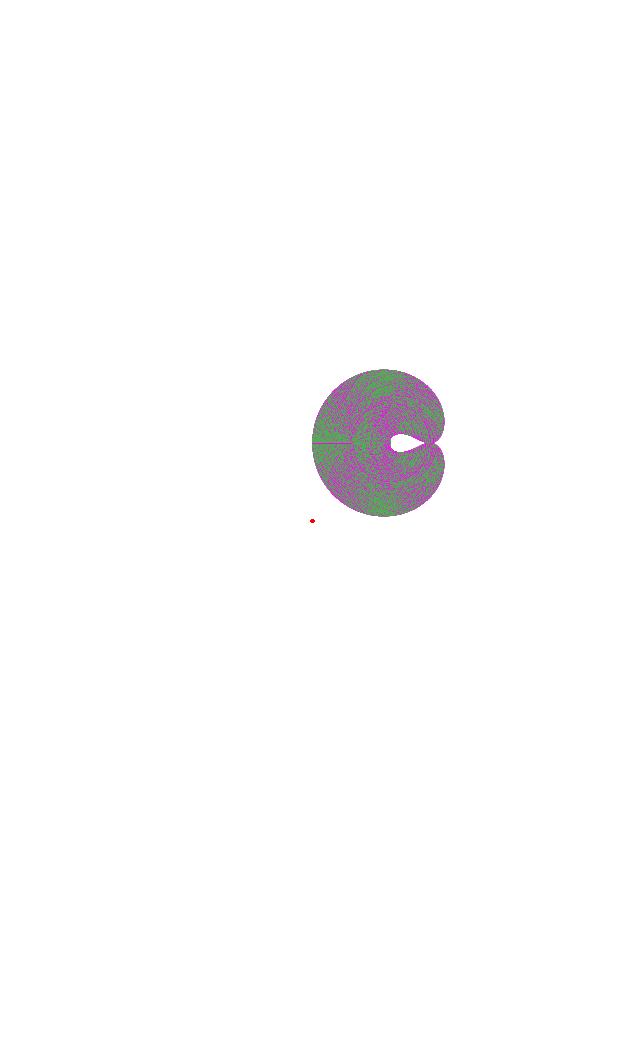
\includegraphics{../python-notebooks/distort.pdf}
  \caption{Distortion of the plane by iterating a function.}\label{fig:distort}
\end{figure}
\begin{figure}[ht]
  \centering
  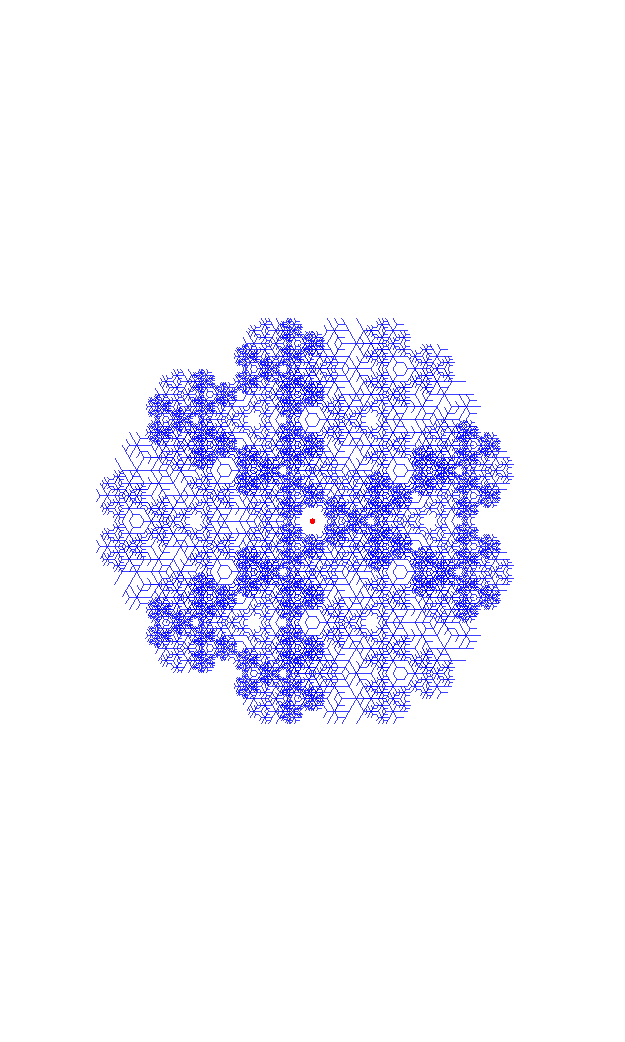
\includegraphics{../python-notebooks/linefractal.pdf}
  \caption{A line fractal from an iterated function system.}\label{fig:linefractal}
\end{figure}
\begin{figure}[ht]
  \centering
  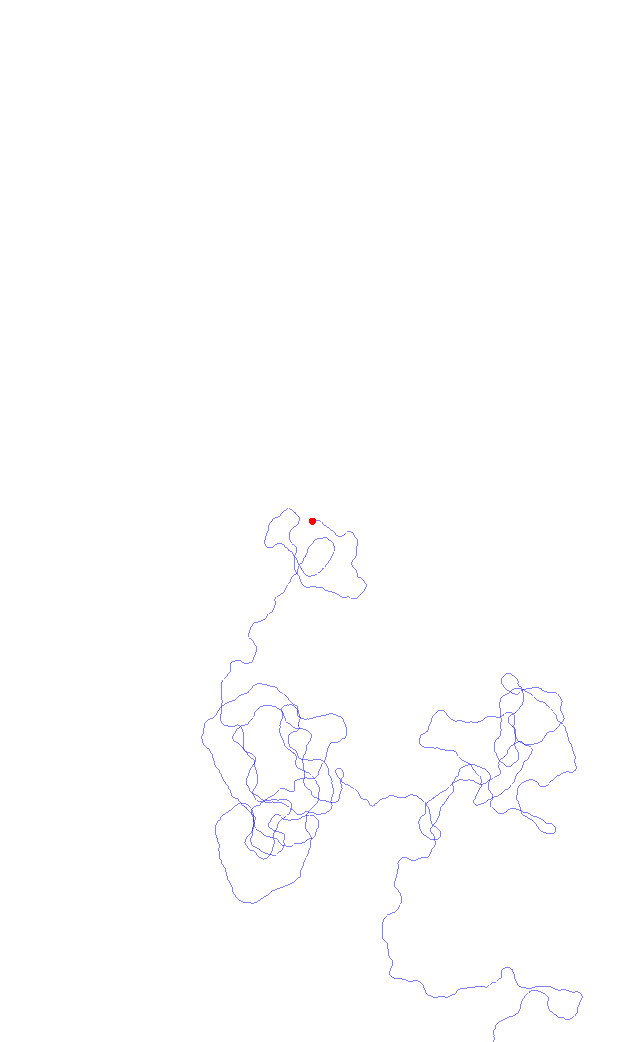
\includegraphics{../python-notebooks/turtle.pdf}
  \caption{Demonstration of turtle drawing.}\label{fig:turtle}
\end{figure}
\begin{figure}[ht]
  \centering
  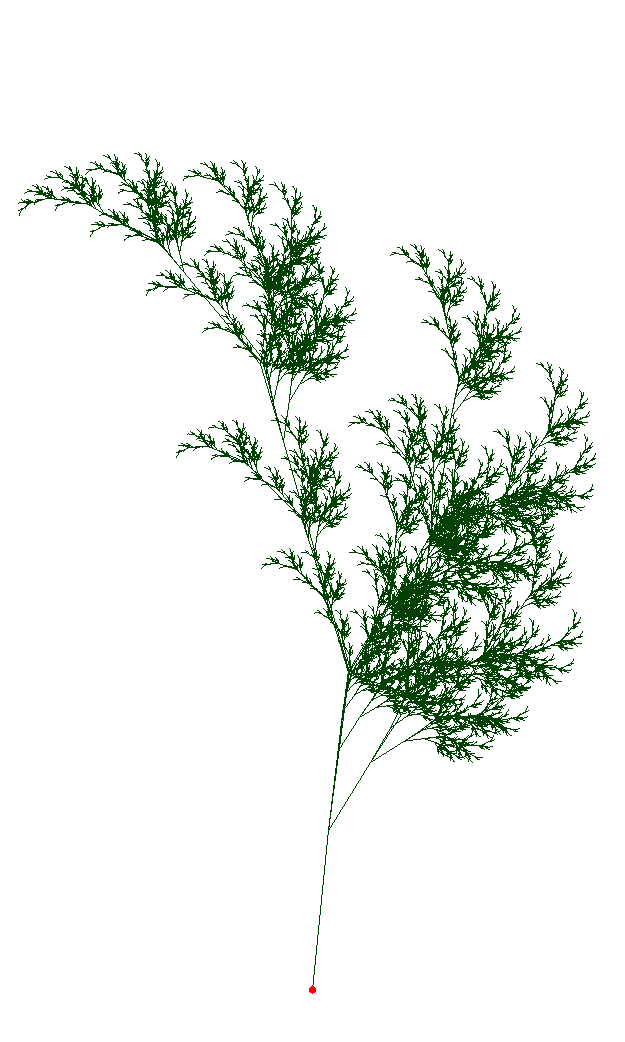
\includegraphics{../python-notebooks/lsystem.pdf}
  \caption{The Barnsley fern Lindenmayer system with some randomness.}\label{fig:lsystem}
\end{figure}
\begin{figure}[ht]
  \centering
  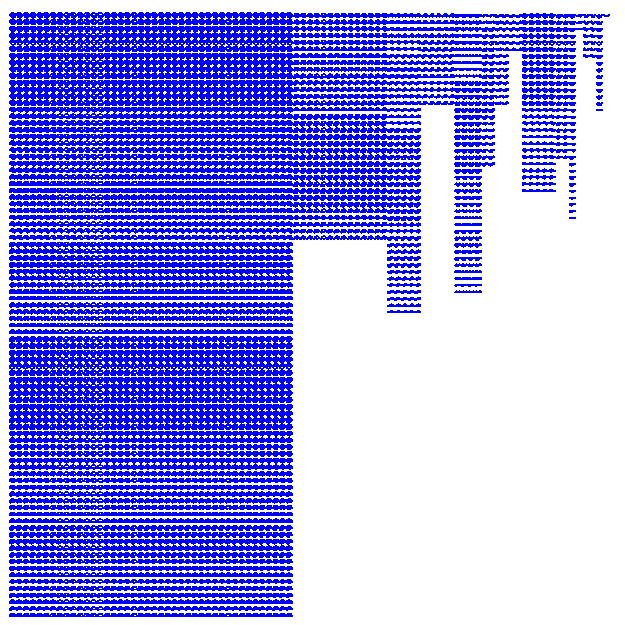
\includegraphics{../python-notebooks/intpartitions_6_grid.pdf}
  \caption{Integer partition shapes. Animals or ghosts are examples of
    \textit{pareidolia}.
    \href{https://web.archive.org/web/20181010091056/http://community.wolfram.com/groups/-/m/t/995095}{%
    Other creatures}
    are found in smoothed out connected regions in random \textsc{bw}
  pixels.}\label{fig:intpartitions}
\end{figure}

\end{document}

